%% template-AutoScaling.tex
%% Author: Zongxu Mu
%% This is the LaTeX template file for Empirical Scaling Analyser (ESA).
%% ESA takes the template, replace variables with their corresponding values,
%%	and generates an output file named AutoScaling.tex.
%% You may compile this file alone without running ESA to see how the output looks like.
%% Variables are surrounded by ``@@''s
%% Supported variable names include:
%%	- algName, e.g., ``WalkSAT/SKC''
%%	- instName, e.g., ``random 3SAT at phase transition''
%%	- models, e.g., ``\\begin{itemize}\n\\item $Exp\\left[a,b\\right]\\left(n\\right)=a\\cdot b^{n}$ \\quad{}(2-parameter exponential);\n\\end{itemize}''
%%	- numBootstrapSamples, the number of bootstrap samples used in the analysis, e.g., 1000
%%	- numSizes, the number of sizes used in the analysis, e.g., 12
%%	- largestSupportSize, e.g., 500
%%	- table-Details-dataset, e.g., ``\\input{table_Details-dataset}''
%%	- table-Details-dataset, e.g., ``\\input{table_Details-dataset}''
%%	- table-Fitted-models, e.g., ``\\begin{tabular}{ccccc} 
\hline 
 &  & \multirow{2}{*}{Model} & RMSE  & RMSE\tabularnewline 
 &  &  & (support)  & (challenge)\tabularnewline 
\hline 
\hline 
\multirow{3}{*}{p15S363} & EXP. Model & $0.95094\times 1.0017^{x}$ & $0.34618$ & $30.319$ \tabularnewline 
 & Poly. Model & $4.3589\times10^{-8}\times x^{2.675}$ & $0.84016$ & $34.759$ \tabularnewline 
 & SQRTEXP. Model & $\mathbf{0.06958\times 1.145^{\sqrt{x}}}$ & $\mathbf{0.39499}$ & $\mathbf{19.033}$ \tabularnewline 
\hline 
\end{tabular} 

''
%%	- figure-fittedModels, e.g., ``\\includegraphics[width=0.8\textwidth]{fittedModels_loglog}''
%%	- supportSizes, the sizes used for fitting the models, e.g., ``200, 250, 300, 350, 400, 450, 500''
%%	- challengeSizes, e.g., ``600, 700, 800, 900, 1000''
%%	- table-Bootstrap-intervals-of-parameters, e.g., ``\\begin{tabular}{cc|cc} 
\hline 
Solver  & Model  & Confidence interval of $a$  & Confidence interval of $b$ \tabularnewline 
\hline 
\multirow{3}{*}{WalkSAT/SKC} & Exp. & $\left[0.0004476,0.0010113\right]$ & $\left[1.007,1.0091\right]$ \tabularnewline 
 & RootExp. & $\left[1.0905\times10^{-5},6.1897\times10^{-5}\right]$ & $\left[1.3243,1.4433\right]$ \tabularnewline 
 & Poly. & $\left[4.5554\times10^{-12},1.011\times10^{-9}\right]$ & $\left[2.7812,3.6834\right]$ \tabularnewline 
\hline 
\end{tabular} 

''
%%	- table-Bootstrap-intervals, e.g., ``\\input{table_Bootstrap-intervals}''
%%	- analysisSummary, e.g., ``observed median running times are consistent with the polynomial scaling model''
\documentclass[british]{article}
\usepackage[T1]{fontenc}
\usepackage[latin9]{inputenc}
\usepackage{geometry}
\geometry{verbose,tmargin=3.5cm,bmargin=3.5cm,lmargin=3cm,rmargin=3cm}
\usepackage{array}
\usepackage{multirow}
\usepackage{amstext}
\usepackage{graphicx}
\usepackage{color}

\newcommand{\medianInterval}[1]{}


\makeatletter

%%%%%%%%%%%%%%%%%%%%%%%%%%%%%% LyX specific LaTeX commands.
%% Because html converters don't know tabularnewline
\providecommand{\tabularnewline}{\\}

%%%%%%%%%%%%%%%%%%%%%%%%%%%%%% User specified LaTeX commands.

\title{On the empirical scaling of running time of p15S363 for solving RUE Instances}
\author{Empirical Scaling Analyser}

\makeatother

\usepackage{babel}
\begin{document}
\maketitle %


\section{Introduction}

This is the automatically generated report on the empirical scaling
of the running time of p15S363 for solving RUE Instances.


\section{Methodology}

\label{sec:Methodology}

% models, model fitting
For our scaling analysis, we considered the following parametric models:
\begin{itemize} 
\item $EXP\left[a,b\right]\left(n\right)=a\times b^{x}$ \quad{}(2-parameter EXP)\item $Poly\left[a,b\right]\left(n\right)=a\times x^{b}$ \quad{}(2-parameter Poly)\item $SQRTEXP\left[a,b\right]\left(n\right)=a\times b^{\sqrt{x}}$ \quad{}(2-parameter SQRTEXP)\end{itemize}
% \begin{itemize}
% \item $Exp\left[a,b\right]\left(n\right)=a\cdot b^{n}$ \quad{}(2-parameter exponential);
% \item $RootExp\left[a,b\right]\left(n\right)=a\cdot b^{\sqrt{n}}$ \quad{}(2-parameter root-exponential);
% \item $Poly\left[a,b\right]\left(n\right)=a\cdot n^{b}$ \quad{}(2-parameter polynomial).
% \end{itemize}
Note that the approach could be easily extended to other scaling models.
For fitting parametric scaling models to observed data, we used the
non-linear least-squares Levenberg-Marquardt algorithm.

% what we fitted the models to, how we assessed model fit
Models were fitted to performance observations in the form of medians
of the distributions of running times over sets of instances for given
$n$, the instance size.
%Compared to the mean, the median has two
%advantages: it is statistically more stable and immune to the presence
%of a certain amount of timed-out runs.
To assess the fit of a given
scaling model to observed data, we used root-mean-square error (RMSE).

\medianInterval{
Due to the instances for which the running times are unknown,
there is uncertainty about the
precise location of the medians of the running time distributions
at each such $n$, and we can only provide bounds on
those medians instead. Closely following \cite{dubois2015on}, we calculate
these bounds based on the best
and worst case scenarios, in which all instances with unknown running times
are easiest or hardest, respectively.
We note that these are not confidence
intervals, since we can guarantee the actual median running
times to lie within them.
We also calculate RMSEs and confidence intervals based on these bounds.
}

% bootstrap confidence intervals
Closely following \cite{hoos2009bootstrap,hoos2014empirical}, we
computed 95\% bootstrap confidence intervals for the performance predictions
obtained from our scaling models, based on 1000 bootstrap samples
per instance set and 1000 automatically fitted variants of each scaling
model.
In the following, we say that a scaling model is in-
consistent with observed data if the bootstrap confidence interval for the observed data
is disjoint from the bootstrap confidence interval for
predicted running times;
\medianInterval{we say that a scaling model is consistent
with observed data, if the interval for observed medians
overlaps with, but is not fully contained within the
bootstrap confidence interval for predicted running times;}
we say that a scaling model is strongly consistent with observed
data, if the observed median is fully contained
within the bootstrap confidence interval for predicted
running times.
Also, we define residue of a model at a given size as the observed
point estimate less the predicated value.

\section{Dataset Description}

The dataset contains running times of the p15S363 algorithm solving
6 sets of instances of different sizes. We split the running times into
two categories, support ($n\leq2000$) and challenge ($n>2000$). The
details of the dataset can be found in Tables \ref{tab:Details-dataset-support}
and \ref{tab:Details-dataset-challenge}.
\begin{table*}
\noindent \begin{centering}
\begin{tabular}{c|cccc} 
\hline 
$n$ & 200 & 250 & 300 & 350 \tabularnewline 
\hline 
\# instances & 601 & 589 & 633 & 558 \tabularnewline 
\# running times & 601 & 589 & 633 & 558 \tabularnewline 
mean & $0.006527$ & $0.01671$ & $0.04785$ & $0.07433$ \tabularnewline 
coefficient of variation & $1.932$ & $2.708$ & $7.148$ & $4.636$ \tabularnewline 
Q(0.1) & $0.000584$ & $0.001108$ & $0.001648$ & $0.002231$ \tabularnewline 
Q(0.25) & $0.000994$ & $0.001882$ & $0.003173$ & $0.004306$ \tabularnewline 
median & $0.002093$ & $0.004457$ & $0.007494$ & $0.01094$ \tabularnewline 
Q(0.75) & $0.005678$ & $0.01213$ & $0.02102$ & $0.02984$ \tabularnewline 
Q(0.9) & $0.01572$ & $0.03676$ & $0.05997$ & $0.0899$ \tabularnewline 
\hline 
\end{tabular} 
\medskip{} 

\begin{tabular}{c|ccc} 
\hline 
$n$ & 400 & 450 & 500 \tabularnewline 
\hline 
\# instances & 579 & 572 & 578 \tabularnewline 
\# running times & 579 & 572 & 578 \tabularnewline 
mean & $0.2162$ & $0.2634$ & $2.171$ \tabularnewline 
coefficient of variation & $8.165$ & $6.233$ & $17.97$ \tabularnewline 
Q(0.1) & $0.003448$ & $0.005009$ & $0.006445$ \tabularnewline 
Q(0.25) & $0.007598$ & $0.01004$ & $0.01438$ \tabularnewline 
median & $0.01825$ & $0.02414$ & $0.03651$ \tabularnewline 
Q(0.75) & $0.05361$ & $0.08692$ & $0.1295$ \tabularnewline 
Q(0.9) & $0.2451$ & $0.3535$ & $0.4501$ \tabularnewline 
\hline 
\end{tabular} 
\medskip{} 


\par\end{centering}

\caption{\label{tab:Details-dataset-support} Details of the running time dataset used as support data for model fitting.}
\end{table*}

\begin{table*}
\noindent \begin{centering}
\begin{tabular}{c|cc} 
\hline 
$n$ & 2500 & 3000 \tabularnewline 
\hline 
\# instances & 100 & 100 \tabularnewline 
\# running times & 100 & 100 \tabularnewline 
mean & $\infty $ & $\infty $ \tabularnewline 
coefficient of variation & $N/A$ & $N/A$ \tabularnewline 
Q(0.1) & $28.7$ & $46.02$ \tabularnewline 
Q(0.25) & $32.01$ & $70.67$ \tabularnewline 
median & $41.9$ & $135$ \tabularnewline 
Q(0.75) & $76.26$ & $249.2$ \tabularnewline 
Q(0.9) & $155.7$ & $\infty $ \tabularnewline 
\hline 
\end{tabular} 
\medskip{} 


\par\end{centering}

\caption{\label{tab:Details-dataset-challenge} Details of the running time dataset used as challenge data for model fitting.}
\end{table*}

%
% Figure \ref{fig:CDFs} shows the distributions of the running times of
% p15S363 solving RUE Instances.
% \begin{figure*}[tb]
% \begin{centering}
% \includegraphics[width=0.8\textwidth]{cdfs}
% % \includegraphics[width=0.8\textwidth]{cdfs}
% \par\end{centering}
%
% \noindent \centering{}\caption{\label{fig:CDFs} Distribution of running times across instance sets for
% p15S363.}
% \end{figure*}
%
%

\section{Empirical Scaling of Solver Performance}

\label{sec:Results}

We first fitted our parametric scaling models to the medians of the running times
of p15S363, as described in Section \ref{sec:Methodology}. The
models were fitted using the medians of the running times for $500\leq n\leq 2000$
(support) and later challenged with the medians of the running times for $2500\leq n\leq 3000$.
This resulted in the models, shown along with RMSEs on support and
challenge data, shown in Table~\ref{tab:Fitted-models}.
\begin{table}[tb]
\begin{centering}
\begin{tabular}{ccccc} 
\hline 
 &  & \multirow{2}{*}{Model} & RMSE  & RMSE\tabularnewline 
 &  &  & (support)  & (challenge)\tabularnewline 
\hline 
\hline 
\multirow{3}{*}{p15S363} & EXP. Model & $0.95094\times 1.0017^{x}$ & $0.34618$ & $30.319$ \tabularnewline 
 & Poly. Model & $4.3589\times10^{-8}\times x^{2.675}$ & $0.84016$ & $34.759$ \tabularnewline 
 & SQRTEXP. Model & $\mathbf{0.06958\times 1.145^{\sqrt{x}}}$ & $\mathbf{0.39499}$ & $\mathbf{19.033}$ \tabularnewline 
\hline 
\end{tabular} 


% \begin{tabular}{ccccc} 
\hline 
 &  & \multirow{2}{*}{Model} & RMSE  & RMSE\tabularnewline 
 &  &  & (support)  & (challenge)\tabularnewline 
\hline 
\hline 
\multirow{3}{*}{p15S363} & EXP. Model & $0.95094\times 1.0017^{x}$ & $0.34618$ & $30.319$ \tabularnewline 
 & Poly. Model & $4.3589\times10^{-8}\times x^{2.675}$ & $0.84016$ & $34.759$ \tabularnewline 
 & SQRTEXP. Model & $\mathbf{0.06958\times 1.145^{\sqrt{x}}}$ & $\mathbf{0.39499}$ & $\mathbf{19.033}$ \tabularnewline 
\hline 
\end{tabular} 


\par\end{centering}

\caption{\label{tab:Fitted-models}Fitted models of the medians of the running times and RMSE
values (in CPU sec). The models yielding more
accurate predictions (as per RMSEs on challenge data) are shown in
boldface.}
\end{table}
In addition, we illustrate the fitted models of p15S363 in Figure~\ref{fig:Fitted-models},
and the residues for the models in Figure~\ref{fig:Fitted-residues}.
\begin{figure}[tb]
\noindent \begin{centering}
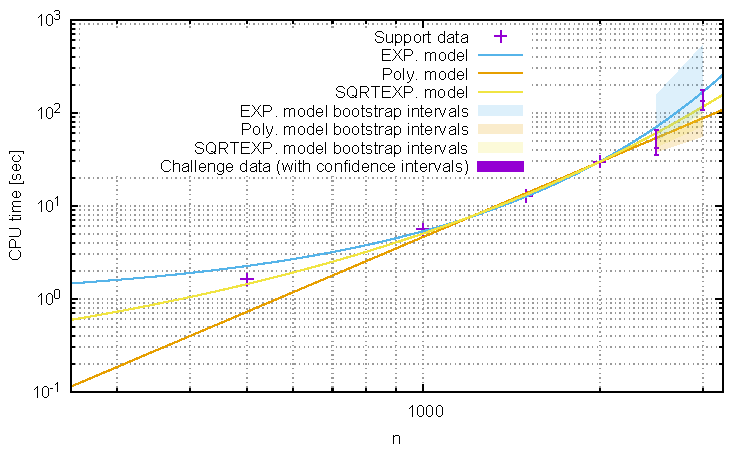
\includegraphics[width=0.8\textwidth]{fittedModels}
% 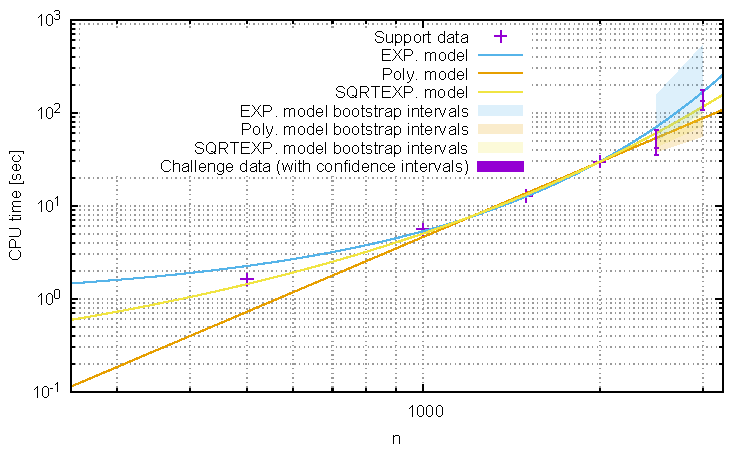
\includegraphics[width=0.8\textwidth]{fittedModels}
\par\end{centering}

\caption{\label{fig:Fitted-models} Fitted models of the medians of the running times.
The models are fitted with the medians of the running times of
p15S363 solving the set of RUE Instances
of $500\leq n\leq 2000$ variables, and are challenged by the medians of the
running times of $2500\leq n\leq 3000$ variables.}
\end{figure}


\begin{figure}[tb]
\noindent \begin{centering}
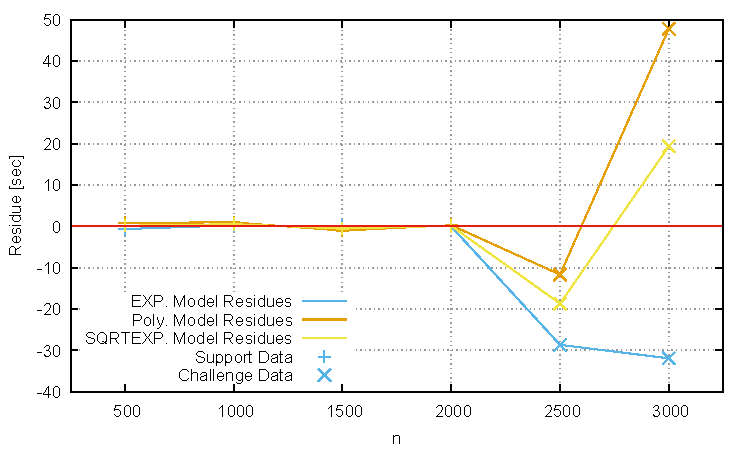
\includegraphics[width=0.8\textwidth]{fittedResidues}
% 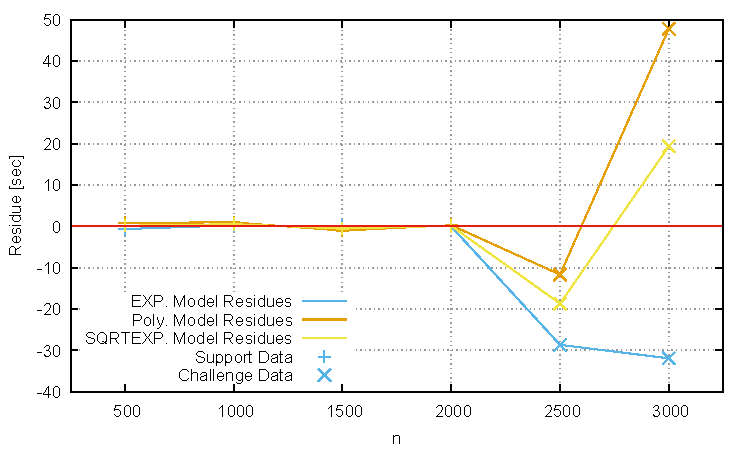
\includegraphics[width=0.8\textwidth]{fittedResidues}
\par\end{centering}

\caption{\label{fig:Fitted-residues} Residues of the fitted models of the medians
of the running times. }
\end{figure}


But how much confidence should we have in these models? Are the RMSEs
small enough that we should accept them? To answer this question,
we assessed the fitted models using the bootstrap approach outlined
in Section~\ref{sec:Methodology}. Table~\ref{tab:Bootstrap-intervals-of-parameters}
shows the bootstrap intervals of the model parameters,
and Table~\ref{tab:Bootstrap-intervals-support}
contains the bootstrap intervals for the support data.
Challenging the models with extrapolation, as shown in
Table~\ref{tab:Bootstrap-intervals-challenge}, it is concluded that
the EXP model tends to over-estimate the data, the Poly model under-estimates the data, and the SQRTEXP model under-estimates the data
(as also illustrated in Figure~\ref{fig:Fitted-models}).
\begin{table*}[tb]
\noindent \begin{centering}
\begin{tabular}{cc|cc} 
\hline 
Solver  & Model  & Confidence interval of $a$  & Confidence interval of $b$ \tabularnewline 
\hline 
\multirow{3}{*}{WalkSAT/SKC} & Exp. & $\left[0.0004476,0.0010113\right]$ & $\left[1.007,1.0091\right]$ \tabularnewline 
 & RootExp. & $\left[1.0905\times10^{-5},6.1897\times10^{-5}\right]$ & $\left[1.3243,1.4433\right]$ \tabularnewline 
 & Poly. & $\left[4.5554\times10^{-12},1.011\times10^{-9}\right]$ & $\left[2.7812,3.6834\right]$ \tabularnewline 
\hline 
\end{tabular} 


% \begin{tabular}{cc|cc} 
\hline 
Solver  & Model  & Confidence interval of $a$  & Confidence interval of $b$ \tabularnewline 
\hline 
\multirow{3}{*}{WalkSAT/SKC} & Exp. & $\left[0.0004476,0.0010113\right]$ & $\left[1.007,1.0091\right]$ \tabularnewline 
 & RootExp. & $\left[1.0905\times10^{-5},6.1897\times10^{-5}\right]$ & $\left[1.3243,1.4433\right]$ \tabularnewline 
 & Poly. & $\left[4.5554\times10^{-12},1.011\times10^{-9}\right]$ & $\left[2.7812,3.6834\right]$ \tabularnewline 
\hline 
\end{tabular} 



\par\end{centering}
\caption{\label{tab:Bootstrap-intervals-of-parameters} 95\% bootstrap intervals
of model parameters for the medians of the running times}
\end{table*}
\begin{table*}[tb]
\noindent \begin{centering}
\begin{tabular}{ccccc}
\hline 
\multirow{2}{*}{Solver} & \multirow{2}{*}{$n$} & Predicted confidence intervals & \multicolumn{2}{c}{Observed median run-time}\tabularnewline
 &  & Exp. model  & Point estimates  & Confidence intervals\tabularnewline
\hline 
\hline 
\multirow{7}{*}{WalkSAT/SKC} & 200 & $\left[0.002754,0.004125\right]$ & $0.002093$ & $\left[0.001899,0.002539\right]$ \tabularnewline 
 & 250 & $\mathbf{\left[0.004279,0.005926\right]}$ & $0.004457$ & $\left[0.003664,0.005377\right]$ \tabularnewline 
 & 300 & $\mathbf{\left[0.006648,0.008532\right]}$\textbf{*} & $0.007494$ & $\left[0.006795,0.008479\right]$ \tabularnewline 
 & 350 & $\mathbf{\left[0.01034,0.01227\right]}$ & $0.01094$ & $\left[0.009792,0.01258\right]$ \tabularnewline 
 & 400 & $\mathbf{\left[0.01563,0.01822\right]}$ & $0.01825$ & $\left[0.01601,0.0201\right]$ \tabularnewline 
 & 450 & $\mathbf{\left[0.0228,0.02791\right]}$ & $0.02414$ & $\left[0.02149,0.02995\right]$ \tabularnewline 
 & 500 & $\mathbf{\left[0.03263,0.04218\right]}$ & $0.03651$ & $\left[0.03177,0.04233\right]$ \tabularnewline 
\hline 
\end{tabular} 

\begin{tabular}{ccccc}
\hline 
\multirow{2}{*}{Solver} & \multirow{2}{*}{$n$} & Predicted confidence intervals & \multicolumn{2}{c}{Observed median run-time}\tabularnewline
 &  & RootExp. model  & Point estimates  & Confidence intervals\tabularnewline
\hline 
\hline 
\multirow{7}{*}{WalkSAT/SKC} & 200 & $\mathbf{\left[0.002052,0.00334\right]}$ & $0.002093$ & $\left[0.001899,0.002539\right]$ \tabularnewline 
 & 250 & $\mathbf{\left[0.003717,0.005335\right]}$ & $0.004457$ & $\left[0.003664,0.005377\right]$ \tabularnewline 
 & 300 & $\mathbf{\left[0.006362,0.008301\right]}$ & $0.007494$ & $\left[0.006795,0.008479\right]$ \tabularnewline 
 & 350 & $\mathbf{\left[0.01049,0.01242\right]}$ & $0.01094$ & $\left[0.009792,0.01258\right]$ \tabularnewline 
 & 400 & $\mathbf{\left[0.01612,0.01876\right]}$ & $0.01825$ & $\left[0.01601,0.0201\right]$ \tabularnewline 
 & 450 & $\mathbf{\left[0.02324,0.02848\right]}$ & $0.02414$ & $\left[0.02149,0.02995\right]$ \tabularnewline 
 & 500 & $\mathbf{\left[0.03229,0.0418\right]}$ & $0.03651$ & $\left[0.03177,0.04233\right]$ \tabularnewline 
\hline 
\end{tabular} 

\begin{tabular}{ccccc}
\hline 
\multirow{2}{*}{Solver} & \multirow{2}{*}{$n$} & Predicted confidence intervals & \multicolumn{2}{c}{Observed median run-time}\tabularnewline
 &  & Poly. model  & Point estimates  & Confidence intervals\tabularnewline
\hline 
\hline 
\multirow{7}{*}{WalkSAT/SKC} & 200 & $\mathbf{\left[0.001369,0.002609\right]}$\textbf{*} & $0.002093$ & $\left[0.001899,0.002539\right]$ \tabularnewline 
 & 250 & $\mathbf{\left[0.003143,0.004819\right]}$ & $0.004457$ & $\left[0.003664,0.005377\right]$ \tabularnewline 
 & 300 & $\mathbf{\left[0.006063,0.00811\right]}$ & $0.007494$ & $\left[0.006795,0.008479\right]$ \tabularnewline 
 & 350 & $\mathbf{\left[0.01061,0.01266\right]}$ & $0.01094$ & $\left[0.009792,0.01258\right]$ \tabularnewline 
 & 400 & $\mathbf{\left[0.01661,0.01927\right]}$ & $0.01825$ & $\left[0.01601,0.0201\right]$ \tabularnewline 
 & 450 & $\mathbf{\left[0.02363,0.02901\right]}$ & $0.02414$ & $\left[0.02149,0.02995\right]$ \tabularnewline 
 & 500 & $\mathbf{\left[0.03187,0.04135\right]}$ & $0.03651$ & $\left[0.03177,0.04233\right]$ \tabularnewline 
\hline 
\end{tabular} 



% \input{table_Bootstrap-intervals}
\par\end{centering}

\caption{\label{tab:Bootstrap-intervals-support} 95\% bootstrap confidence intervals
for the medians of the running time predictions and observed running times on RUE Instances.
The instance sizes shown here are those used for fitting the models.
Bootstrap intervals on predictions that are weakly consistent
with the observed point estimates are shown in boldface,
those that are consistent are marked by plus signs ({+}),
and those that fully contain the confidence intervals on
observations are marked by asterisks ({*}).}
\end{table*}

\begin{table*}[tb]
\noindent \begin{centering}
\begin{tabular}{ccccc}
\hline 
\multirow{2}{*}{Solver} & \multirow{2}{*}{$n$} & Predicted confidence intervals & \multicolumn{2}{c}{Observed median run-time}\tabularnewline
 &  & EXP. model  & Point estimates  & Confidence intervals\tabularnewline
\hline 
\hline 
\multirow{2}{*}{p15S363} & 2500 & $\mathbf{\left[50.14,154\right]}$ & $41.9$ & $\left[35.35,64.72\right]$ \tabularnewline 
 & 3000 & $\mathbf{\left[102.2,525.1\right]}$\textbf{*} & $135$ & $\left[107.2,177.2\right]$ \tabularnewline 
\hline 
\end{tabular} 

\begin{tabular}{ccccc}
\hline 
\multirow{2}{*}{Solver} & \multirow{2}{*}{$n$} & Predicted confidence intervals & \multicolumn{2}{c}{Observed median run-time}\tabularnewline
 &  & Poly. model  & Point estimates  & Confidence intervals\tabularnewline
\hline 
\hline 
\multirow{2}{*}{p15S363} & 2500 & $\mathbf{\left[38.07,54.13\right]}$\textbf{\#} & $41.9$ & $\left[35.35,64.72\right]$ \tabularnewline 
 & 3000 & $\left[55.77,89.02\right]$ & $135$ & $\left[107.2,177.2\right]$ \tabularnewline 
\hline 
\end{tabular} 

\begin{tabular}{ccccc}
\hline 
\multirow{2}{*}{Solver} & \multirow{2}{*}{$n$} & Predicted confidence intervals & \multicolumn{2}{c}{Observed median run-time}\tabularnewline
 &  & SQRTEXP. model  & Point estimates  & Confidence intervals\tabularnewline
\hline 
\hline 
\multirow{2}{*}{p15S363} & 2500 & $\mathbf{\left[42.94,61.24\right]}$ & $41.9$ & $\left[35.35,64.72\right]$ \tabularnewline 
 & 3000 & $\mathbf{\left[72.4,118.1\right]}$ & $135$ & $\left[107.2,177.2\right]$ \tabularnewline 
\hline 
\end{tabular} 



% \input{table_Bootstrap-intervals}
\par\end{centering}

\caption{\label{tab:Bootstrap-intervals-challenge} 95\% bootstrap confidence intervals
for the medians of the running time predictions and observed running times on RUE Instances.
The instance sizes shown here are larger than those used for fitting the models.
Bootstrap intervals on predictions that are weakly consistent
with the observed data are shown in boldface,
\medianInterval{those that are consistent are marked by plus signs ({+}),}
those that are strongly consistent are marked
by sharps ({\#}),
and those that fully contain the confidence intervals on
observations are marked by asterisks ({*}).}
\end{table*}


\section{Conclusion}

In this report, we presented an empirical analysis of the scaling
behaviour of p15S363 on RUE Instances. We found
the EXP model tends to over-estimate the data, the Poly model under-estimates the data, and the SQRTEXP model under-estimates the data.

\bibliographystyle{plain}
\begin{thebibliography}{1}

\bibitem{dubois2015on}
J{\'e}r{\'e}mie Dubois-Lacoste, Holger~H. Hoos, and Thomas St{\"u}tzle.
\newblock On the empirical scaling behaviour of state-of-the-art local search
algorithms for the euclidean tsp.
\newblock In {\em GECCO}. ACM, 2015.

\bibitem{hoos2009bootstrap}
Holger~H Hoos.
\newblock A bootstrap approach to analysing the scaling of empirical run-time
data with problem size.
\newblock Technical report, Technical Report TR-2009-16, University of British
Columbia, 2009.

\bibitem{hoos2014empirical}
Holger~H Hoos and Thomas St{\"u}tzle.
\newblock On the empirical scaling of run-time for finding optimal solutions to
the travelling salesman problem.
\newblock {\em European Journal of Operational Research}, 238(1):87--94, 2014.

\end{thebibliography}

\end{document}
